% Adapted from templates/latex/报告模板.zip (XeLaTeX, unofficial CUHK-SZ report style).
\usepackage{fontspec,xeCJK}
\setmainfont{texgyretermes}[Extension=.otf,UprightFont=*-regular,BoldFont=*-bold,ItalicFont=*-italic,BoldItalicFont=*-bolditalic]
\setsansfont{texgyreheros}[Extension=.otf,UprightFont=*-regular,BoldFont=*-bold,ItalicFont=*-italic,BoldItalicFont=*-bolditalic]
\setmonofont{Menlo}[Scale=0.84]
\setCJKmainfont{Songti SC}[AutoFakeBold=2]
\setCJKsansfont{Hiragino Sans GB}
\setCJKmonofont{Hiragino Sans GB}
\usepackage{microtype}
\usepackage[a4paper,margin=25mm,headheight=22pt,headsep=8mm,footskip=12mm]{geometry}
\usepackage{graphicx,amsmath,amssymb,mathtools}
\usepackage{booktabs,longtable,tabularx,array,calc}
\usepackage{enumitem,listings,fvextra,caption,fancyhdr,lastpage,titlesec,xcolor}
\usepackage{etoolbox,float,adjustbox,pdflscape,needspace,soul,newunicodechar,seqsplit}
\usepackage{tikz}
\usetikzlibrary{arrows.meta,positioning,calc,fit,shapes.geometric,shapes.multipart,matrix}
\usepackage[unicode,pdfencoding=auto,bookmarksnumbered=false]{hyperref}
\definecolor{CUHKPurple}{HTML}{5C2267}
\definecolor{CUHKGold}{HTML}{C99A2E}
\definecolor{Ink}{HTML}{20242B}
\definecolor{Muted}{HTML}{626B75}
\definecolor{Rule}{HTML}{D8DCE0}
\definecolor{CodeBg}{HTML}{F5F6F8}
\color{Ink}
\hypersetup{colorlinks=true,linkcolor=CUHKPurple,urlcolor=CUHKPurple,pdfauthor={CSC5041 Personal Study Materials},pdftitle={CSC5041 Revision Materials}}
\setlist{leftmargin=*,itemsep=2pt,topsep=4pt}
\setlength{\parindent}{0pt}
\setlength{\parskip}{5pt}
\setlength{\emergencystretch}{3em}
\linespread{1.08}
\setcounter{secnumdepth}{0}
\setcounter{tocdepth}{2}
\titleformat{\section}{\sffamily\LARGE\bfseries\color{CUHKPurple}}{}{0pt}{}
\titleformat{\subsection}{\sffamily\large\bfseries\color{CUHKPurple}}{}{0pt}{}
\titleformat{\subsubsection}{\sffamily\normalsize\bfseries\color{Ink}}{}{0pt}{}
\titlespacing*{\section}{0pt}{1em}{0.65em}
\titlespacing*{\subsection}{0pt}{1em}{0.4em}
\titlespacing*{\subsubsection}{0pt}{0.7em}{0.25em}
\captionsetup{font=small,labelfont={bf,color=CUHKPurple},labelsep=period}
\pagestyle{fancy}\fancyhf{}
\fancyhead[L]{\sffamily\small\color{Muted}CSC5041 · Database Systems}
\fancyhead[R]{\sffamily\small\color{Muted}\VolumeShort}
\fancyfoot[L]{\sffamily\scriptsize\color{Muted}The Chinese University of Hong Kong, Shenzhen}
\fancyfoot[R]{\sffamily\scriptsize\color{Muted}\thepage\ / \pageref*{LastPage}}
\renewcommand{\headrulewidth}{0.4pt}
\newcommand{\VolumeShort}{Weeks 1--5}
\fancypagestyle{cover}{\fancyhf{}\fancyfoot[R]{\sffamily\small 2026-10-20}\renewcommand{\headrulewidth}{0pt}}
\newcommand{\StudyCover}[3]{%
 \thispagestyle{cover}
 \noindent\begin{minipage}[c]{0.12\textwidth}
\includegraphics[width=0.82\linewidth]{assets/CUHK_Logo.png}\end{minipage}%
 \begin{minipage}[c]{0.85\textwidth}{\sffamily\bfseries\large The Chinese University of Hong Kong, Shenzhen}\par{\sffamily\small\color{Muted}Personal study materials · Unofficial}\end{minipage}
 \par\vspace{12pt}{\color{CUHKGold}\rule{\linewidth}{1.2pt}}\par\vspace{20mm}
 {\sffamily\bfseries\Huge\color{CUHKPurple}#1}\par\vspace{9mm}
 {\sffamily\LARGE #2}\par\vspace{5mm}{\large\color{Muted}#3}\par
 \vfill{\small Adapted from the supplied academic report template.\par Original teaching materials remain unchanged.\par LaTeX edition: 20 October 2026.}\clearpage}
\lstdefinestyle{studysql}{language=SQL,basicstyle=\ttfamily\small,keywordstyle=\color{CUHKPurple}\bfseries,stringstyle=\color{CUHKGold!65!black},commentstyle=\color{Muted},backgroundcolor=\color{CodeBg},frame=single,rulecolor=\color{Rule},breaklines=true,breakatwhitespace=false,columns=fullflexible,keepspaces=true,showstringspaces=false,tabsize=4,aboveskip=8pt,belowskip=8pt}
\lstset{style=studysql}
\DefineVerbatimEnvironment{StudyCode}{Verbatim}{breaklines=true,breakanywhere=true,fontsize=\small,frame=single,rulecolor=\color{Rule},framesep=6pt,baselinestretch=1.1}
\newcommand{\tightlist}{\setlength{\itemsep}{0pt}\setlength{\parskip}{0pt}}
\newcommand{\passthrough}[1]{#1}
\newcommand{\pandocbounded}[1]{\begin{adjustbox}{max width=\linewidth,max totalheight=.78\textheight,keepaspectratio}#1\end{adjustbox}}
\newcommand{\StudyFormula}[1]{\par\noindent\begin{adjustbox}{max width=\linewidth}\(\displaystyle #1\)\end{adjustbox}\par}
\newcommand{\StudyVisual}[2]{\begin{figure}[H]\centering\StudyDiagram{#1}{#2}\end{figure}}
\newcommand{\StudyLandscapeER}{\clearpage\begin{landscape}\thispagestyle{empty}\begin{center}{\sffamily\large\bfseries\color{CUHKPurple}Tutorial 1: complete ER diagram}\par\vspace{4mm}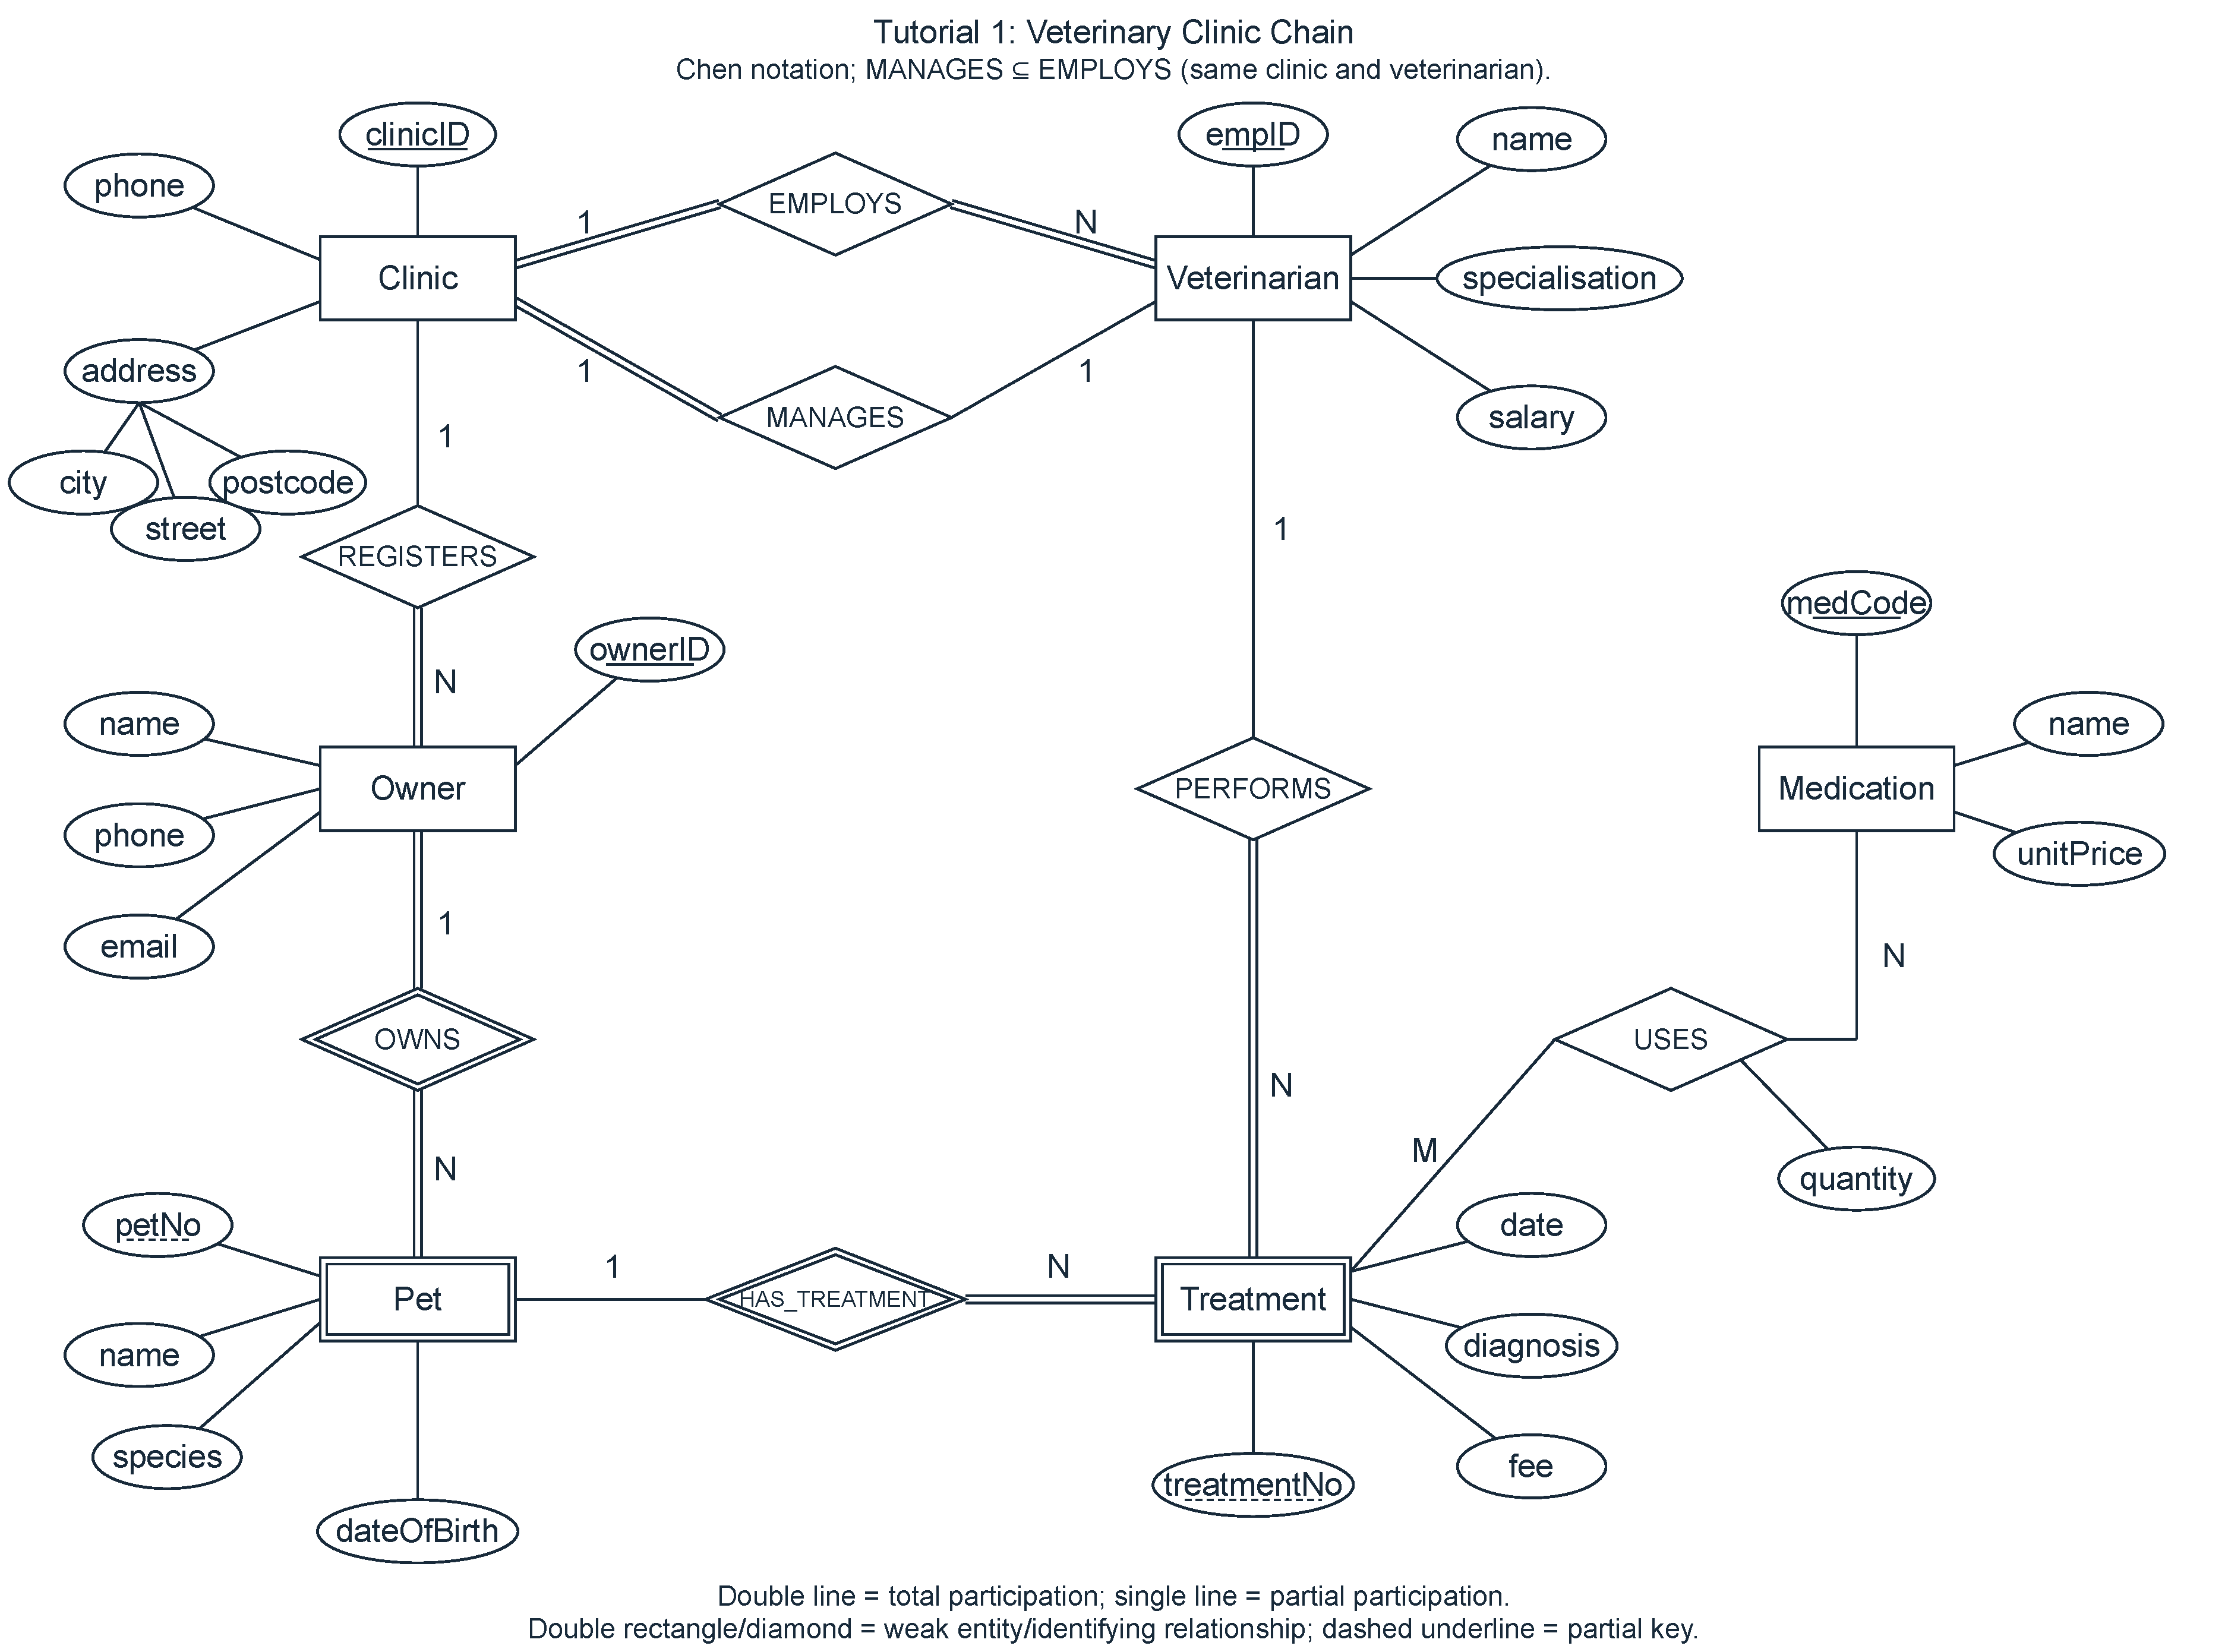
\includegraphics[width=\linewidth,height=.86\textheight,keepaspectratio]{figures/tutorial1_er.pdf}\end{center}\end{landscape}\clearpage}
\setlength{\tabcolsep}{4pt}
\renewcommand{\arraystretch}{1.17}
\AtBeginEnvironment{longtable}{\small}
\setlength{\LTleft}{0pt}\setlength{\LTright}{0pt}
\newunicodechar{σ}{\ensuremath{\sigma}}
\newunicodechar{π}{\ensuremath{\pi}}
\newunicodechar{ρ}{\ensuremath{\rho}}
\newunicodechar{γ}{\ensuremath{\gamma}}
\newunicodechar{θ}{\ensuremath{\theta}}
\newunicodechar{⋈}{\ensuremath{\bowtie}}
\newunicodechar{÷}{\ensuremath{\div}}
\newunicodechar{∀}{\ensuremath{\forall}}
\newunicodechar{∃}{\ensuremath{\exists}}
\newunicodechar{∈}{\ensuremath{\in}}
\newunicodechar{∉}{\ensuremath{\notin}}
\newunicodechar{⊆}{\ensuremath{\subseteq}}
\newunicodechar{∪}{\ensuremath{\cup}}
\newunicodechar{∩}{\ensuremath{\cap}}
\newunicodechar{∧}{\ensuremath{\land}}
\newunicodechar{∨}{\ensuremath{\lor}}
\newunicodechar{¬}{\ensuremath{\neg}}
\newunicodechar{≠}{\ensuremath{\ne}}
\newunicodechar{∅}{\ensuremath{\varnothing}}
\newunicodechar{≤}{\ensuremath{\le}}
\newunicodechar{≥}{\ensuremath{\ge}}
\newunicodechar{×}{\ensuremath{\times}}
\newunicodechar{→}{\ensuremath{\rightarrow}}
\newunicodechar{←}{\ensuremath{\leftarrow}}
\newunicodechar{⇒}{\ensuremath{\Longrightarrow}}
\newunicodechar{−}{\ensuremath{-}}
\newunicodechar{✓}{\ensuremath{\checkmark}}
\newunicodechar{☐}{\ensuremath{\square}}
\newunicodechar{☑}{\ensuremath{\boxtimes}}
% Editable teaching diagrams. Examples reuse Chapters 01--06; no measured data.
% Requires tikz, amsmath, amssymb; colors are defined by the document preamble.
\newcommand{\SDtext}[2]{\ifx\SDlang\SDzh #1\else #2\fi}
\newcommand{\StudyDiagram}[2]{\begingroup
  \edef\SDlang{#2}\def\SDzh{zh}%
  \tikzset{sd box/.style={draw=CUHKPurple,rounded corners=3pt,fill=CUHKPurple!4,align=center,inner sep=7pt,font=\fontsize{10}{13}\selectfont},sd arrow/.style={-{Stealth[length=2mm]},thick,draw=CUHKPurple},sd note/.style={align=center,text=Muted,font=\fontsize{9}{12}\selectfont},sd table/.style={draw=Rule,fill=CodeBg,inner sep=6pt,align=center,font=\fontsize{10}{13}\selectfont}}%
  \csname SDdiagram#1\endcsname
\endgroup}

\newcommand{\SDdiagramschemas}{%
\begin{tikzpicture}[node distance=9mm]
\node[sd box,text width=11.8cm] (e) {\SDtext{外模式：不同用户的视图}{External schemas: different user views}\\\texttt{Student view}\quad|\quad\texttt{Registrar view}};
\node[sd box,text width=11.8cm,below=of e] (c) {\SDtext{概念模式：整个数据库的逻辑结构}{Conceptual schema: database-wide logical structure}\\\texttt{Student(sid,name,major), Course(...), Enrolment(...)}};
\node[sd box,text width=11.8cm,below=of c] (i) {\SDtext{内模式：文件、页、索引与存储组织}{Internal schema: files, pages, indexes and storage organization}};
\draw[sd arrow] (e)--(c);\draw[sd arrow] (c)--(i);
\node[sd note,below=8mm of i,text width=12.6cm] {\SDtext{逻辑独立性：改变概念模式，保持外模式及应用不变。\\物理独立性：改变内模式，保持概念模式不变。}{Logical independence: change conceptual schema; preserve external schemas/applications.\\Physical independence: change internal schema; preserve conceptual schema.}};
\end{tikzpicture}}

\newcommand{\SDdiagramdbms}{%
\begin{tikzpicture}[node distance=7mm]
\node[sd box,text width=11cm] (a) {\SDtext{用户／应用程序}{User / application}\quad\texttt{SELECT ...}};
\node[sd box,text width=11cm,below=of a] (q) {\SDtext{查询处理器：解析、优化、执行}{Query processor: parse, optimize, execute}};
\node[sd box,text width=11cm,below=of q] (s) {\SDtext{存储管理器：缓冲区、文件与索引访问}{Storage manager: buffers, files and index access}};
\node[sd box,text width=11cm,below=of s] (d) {\SDtext{数据库文件＋系统目录（元数据）}{Database files + system catalog (metadata)}};
\draw[sd arrow] (a)--(q);\draw[sd arrow] (q)--(s);\draw[sd arrow] (s)--(d);
\node[sd note,text width=12cm,below=7mm of d] {\SDtext{简化的概念流程；权限、完整性、并发与恢复机制贯穿请求处理。}{Simplified conceptual flow; authorization, integrity, concurrency and recovery support request handling.}};
\end{tikzpicture}}

\newcommand{\SDdiagramweak}{%
\begin{tikzpicture}[node distance=10mm]
\node[sd box,text width=11.4cm] (b) {\textbf{Building}\quad\SDtext{完整键}{Full key}: $\{buildingID\}$};
\node[sd box,text width=11.4cm,below=of b] (r) {\textbf{Room}\quad\SDtext{局部键}{Partial key}: $\{roomNo\}$\\\SDtext{完整键}{Full key}: $\{buildingID,roomNo\}$};
\node[sd box,text width=11.4cm,below=of r] (d) {\textbf{Desk}\quad\SDtext{局部键}{Partial key}: $\{deskNo\}$\\\SDtext{完整键}{Full key}: $\{buildingID,roomNo,deskNo\}$};
\draw[sd arrow] (b)-- node[right,sd note]{\SDtext{继承所有者的完整键}{Carry owner's full key}} (r);
\draw[sd arrow] (r)-- node[right,sd note]{\SDtext{继承所有者的完整键}{Carry owner's full key}} (d);
\node[sd note,text width=12.6cm,below=7mm of d] {\SDtext{自编示例。房号只在楼内唯一，桌号只在房间内唯一。\\Desk 的外键为 $(buildingID,roomNo)$，不能只保留 $roomNo$。}{Original example. Room numbers are local to a building; desk numbers are local to a room.\\Desk references Room with $(buildingID,roomNo)$, not $roomNo$ alone.}};
\end{tikzpicture}}

\newcommand{\SDdiagramintegrity}{%
\begin{tikzpicture}
\node[sd table] (s) at (0,0) {\textbf{Student}\\\begin{tabular}{cc}\underline{sid}&name\\\hline S01&Amy\\S02&Ben\end{tabular}};
\node[sd table] (e) at (7.3,0) {\textbf{Enrolment}\\\begin{tabular}{cc}\underline{sid}&\underline{cid}\\\hline S01&C01\\S01&C02\end{tabular}};
\draw[sd arrow] (e.west)-- node[above,sd note]{\texttt{FK: sid $\to$ sid}} (s.east);
\node[sd note,text width=4.6cm] at (0,-2.15) {\SDtext{主键：唯一且非空}{Primary key: unique and non-NULL}\\$PK(Student)=\{sid\}$};
\node[sd note,text width=6cm] at (7.3,-2.15) {\SDtext{复合主键：整组唯一；sid 可以重复}{Composite PK: pair unique; sid may repeat}\\$PK(Enrolment)=\{sid,cid\}$};
\node[sd box,text width=11.7cm] at (3.6,-4.1) {$\pi_{sid}(Enrolment)\subseteq\pi_{sid}(Student)$\\\SDtext{本例 sid 属于主键，故非空；一般外键是否可空取决于约束。}{Here sid is part of the PK, so non-NULL; a general FK's nullability depends on constraints.}};
\node[sd note,text width=12cm] at (3.6,-5.7) {\SDtext{自编示例；仅展示 sid 引用。cid 还需引用 Course 的键。}{Original example; only the sid reference is shown. cid must also reference Course's key.}};
\end{tikzpicture}}

\newcommand{\SDdiagrammapping}{%
\begin{tikzpicture}
\node[sd box,text width=11.8cm] (a) at (0,0) {\textbf{1:N}\quad\texttt{Department}\ $1\;\text{---}\;N$\ \texttt{Employee}\\\texttt{Department(\underline{deptID}, name)}\\\texttt{Employee(\underline{empID}, name, deptID)}};
\node[sd note,text width=12cm] at (0,-1.65) {$Employee.deptID\longrightarrow Department.deptID$\\\SDtext{外键放 N 侧；若 Employee 全参与，再加 NOT NULL。}{Place FK on the N side; add NOT NULL if Employee participation is total.}};
\node[sd box,text width=11.8cm] (b) at (0,-3.45) {\textbf{M:N}\quad\texttt{Student}\ $M\;\text{---}\;N$\ \texttt{Course}\\\texttt{Enrolment(\underline{sid}, \underline{cid})}\quad $PK=\{sid,cid\}$};
\node[sd note,text width=12cm] at (0,-5) {$Enrolment.sid\to Student.sid\qquad Enrolment.cid\to Course.cid$\\\SDtext{建立关联关系；关系属性也放在此处。外键本身不保证两端全参与。}{Create an association relation; put relationship attributes here. FKs alone do not ensure total participation.}};
\node[sd note,text width=12cm] at (0,-6.1) {\SDtext{自编简化示例；假设同一学生与课程最多关联一次。}{Original simplified example; assume at most one association per student--course pair.}};
\end{tikzpicture}}

\newcommand{\SDdiagramoperators}{%
\begin{tikzpicture}
\node[sd table] (c) at (0,0) {\textbf{Course}\\\begin{tabular}{ccc}cid&dept&credits\\\hline C1&CS&4\\C2&CS&3\\C3&Math&4\end{tabular}};
\node[sd table] (s) at (7.6,1.3) {\begin{tabular}{ccc}cid&dept&credits\\\hline C1&CS&4\end{tabular}};
\node[sd table] (p) at (7.6,-1.4) {\begin{tabular}{c}dept\\\hline CS\\Math\end{tabular}};
\draw[sd arrow] (c.north east)--node[above,sloped,sd note]{$\sigma_{dept='CS'\,\land\,credits>3}$}(s.west);
\draw[sd arrow] (c.south east)--node[below,sloped,sd note]{$\pi_{dept}$}(p.west);
\node[sd note,text width=12cm] at (3.6,-3) {\SDtext{选择：筛行，保留所有列。投影：选列，并消除重复。\\采用第 05 章数据；为图示省略 title 列。}{Selection: filter rows, keep all columns. Projection: retain columns and eliminate duplicates.\\Chapter 05 data; the title column is omitted for display.}};
\end{tikzpicture}}

\newcommand{\SDdiagramdivision}{%
\begin{tikzpicture}
\node[sd table] at (0,0) {\textbf{Takes}\quad$R(sid,cid)$\\\begin{tabular}{cc}sid&cid\\\hline S1&C1\\S1&C2\\S2&C1\\S2&C3\\S3&C3\end{tabular}};
\node[sd table] at (4.25,0.6) {\textbf{Target}\quad$S(cid)$\\\begin{tabular}{c}cid\\\hline C1\\C2\end{tabular}};
\node[sd table] at (9,0.6) {\SDtext{结果}{Result}\quad$R\div S$\\\begin{tabular}{c}sid\\\hline S1\end{tabular}};
\draw[sd arrow] (5.95,0.6)--node[above,sd note]{$\forall cid\in S$}(7.4,0.6);
\node[sd box,text width=11.8cm] at (4.4,-2.6) {$R\div S=\{s\in\pi_{sid}(R)\mid\forall c\in S,\ (s,c)\in R\}$\\\SDtext{覆盖每一门目标课程；允许额外课程；重复不能弥补缺项。}{Cover every target course; extra courses are allowed; duplicates cannot fill a gap.}};
\node[sd note,text width=12cm] at (4.4,-4) {\SDtext{沿用第 05 章数据。S2 缺 C2；S3 缺 C1、C2。\\候选来自 $\pi_{sid}(R)$，因此 S4 不在除法的候选域内。}{Chapter 05 data. S2 lacks C2; S3 lacks C1 and C2.\\Candidates come from $\pi_{sid}(R)$, so S4 is outside this division's candidate domain.}};
\end{tikzpicture}}

\newcommand{\SDdiagramsqlflow}{%
\begin{tikzpicture}[node distance=5mm]
\node[sd box,text width=10.6cm] (f) {\texttt{FROM / JOIN}\quad\SDtext{形成输入行}{Form input rows}};
\node[sd box,text width=10.6cm,below=of f] (w) {\texttt{WHERE}\quad\SDtext{筛选行：只保留 TRUE}{Filter rows: retain TRUE only}};
\node[sd box,text width=10.6cm,below=of w] (g) {\texttt{GROUP BY / aggregation}\quad\SDtext{形成组并聚合}{Form groups and aggregate}};
\node[sd box,text width=10.6cm,below=of g] (h) {\texttt{HAVING}\quad\SDtext{筛选组：只保留 TRUE}{Filter groups: retain TRUE only}};
\node[sd box,text width=10.6cm,below=of h] (s) {\texttt{SELECT $\to$ DISTINCT $\to$ ORDER BY}\quad\SDtext{输出}{Output}};
\draw[sd arrow] (f)--(w);\draw[sd arrow] (w)--(g);\draw[sd arrow] (g)--(h);\draw[sd arrow] (h)--(s);
\node[sd note,text width=12.1cm,below=6mm of s] {\SDtext{普通查询的逻辑阶段，不是强制的物理执行顺序。\\WHERE 不能直接使用同层的 AVG(score)；HAVING 可筛选聚合结果。}{Logical stages for ordinary queries, not a mandatory physical execution order.\\WHERE cannot directly use same-level AVG(score); HAVING can filter aggregate results.}};
\end{tikzpicture}}

\newcommand{\SDdiagramnull}{%
\begin{tikzpicture}
\node[sd box,text width=11.5cm] at (0,1.5) {\texttt{WHERE score >= 80}};
\node[sd table] (t) at (-4,0) {$score=90$\\\textbf{TRUE}};
\node[sd table] (f) at (0,0) {$score=60$\\\textbf{FALSE}};
\node[sd table] (u) at (4,0) {$score=\mathrm{NULL}$\\\textbf{UNKNOWN}};
\node[sd box] (keep) at (-4,-1.8) {\SDtext{保留}{Retain}};
\node[sd box] (reject) at (2,-1.8) {\SDtext{舍弃}{Reject}};
\draw[sd arrow] (t)--(keep);\draw[sd arrow] (f)--(reject);\draw[sd arrow] (u)--(reject);
\node[sd note,text width=12cm] at (0,-3.1) {\SDtext{FALSE 与 UNKNOWN 是不同逻辑值，但 WHERE 都不保留。\\检查空值应使用 IS NULL，而非 = NULL。数值为自编示例。}{FALSE and UNKNOWN differ logically, but WHERE retains neither.\\Use IS NULL to test for NULL, not = NULL. Numbers are original teaching examples.}};
\end{tikzpicture}}

